\documentclass[../MaxHughesThesis.tex]{subfiles}

\begin{document}
After the half-life measurement was completed, the next step was to use the shape of the spectrum to deduce Fierz term. 
In order to get a measurement of the Fierz term, the spectrum shape needed to be carefully described.
In addition to all the theoretical corrections, the effect of bremsstrahlung and the efficiency of the detectors needed to be accounted for.
This is important to account for effect of the gamma ray after the filtering.
The way this was done was with a GEANT4 simulation \cite{Ago03}.
The most updated copy of the code can be found at https://github.com/maximilian29631/Geant4for20F/.


\section{GEANT4 Monte Carlo}
The corrected beta energy spectrum was fed as input to a Monte Carlo.
The program used to model the detectors was GEANT4 version 10.04.02.
In order to use the program, a model of the detector set-up and the initial energies of the primary particles need to be introduced.  

\subsection{Detector Geometry}
A source of the detector geometry were the technical drawings of detectors. 
A drawing of the CsI(Na) implant detector is shown in figure \ref{fig:ImplantTech}
This drawing was the basis of the detector geometry fed into the simulation.

\begin{figure}[!htb]
	\centerline{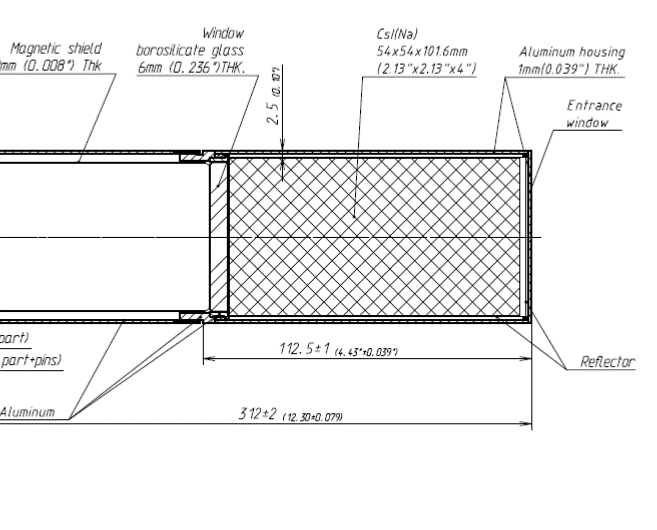
\includegraphics[width=0.78\textwidth]{ImplantDrawing.png}}
	\caption{A techincal drawing of the CsI(Na) implant detector}
	\label{fig:ImplantTech}
\end{figure}

The geometry of the detector set-up was programmed into the simulation.
The implant detector was modeled as a square prism of CsI.
The square prism was 101.6 cm deep with a 5.4 cm square base.
Around the square prism there was an empty layer.
Along the sides, the empty layer was 1.5 mm thick.
On the front and back of the detector, the empty layer was 3.64 mm thick.
After the empty layer, a 1 mm aluminum can surrounded the detector on all sides.  
The center of this detector was placed at the center of the simulation.

The four large gamma detectors also square prisms.
The active volume was 79.5 mm by 79.5 mm by 76.2 mm.
It was also made of CsI.
An empty layer was also added to the gamma detectors.
The empty layer on the sides was also 1.5 mm thick, just like the implant detector.
On the front, however, the empty layer was 2.92 mm thick.
On top of this, the can of aluminum, 1 mm thick on all sides of the detector was added.
The four detectors were arranged in a cross.
The detectors were oriented in such a way that the square face of the CsI crystal faced the implant detector. 
The edge of each of the large gamma detectors was placed 25.4 mm away from the front edge of the implant detector.
This modeled how the implant detector was recessed in the experiment.

A visualization of the CsI crystals in GEANT4 is shown in figure \ref{fig:GEANT4Det}

\begin{figure}[!htb]
	\centerline{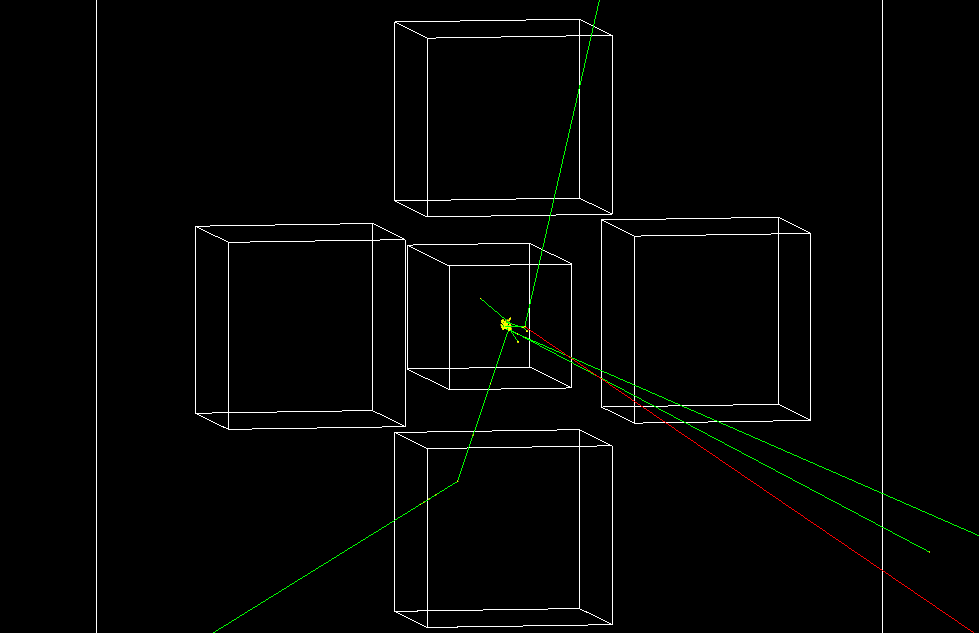
\includegraphics[width=0.78\textwidth]{GEANT4WithoutAl.png}}
	\caption{The detector geometry inside GEANT4}
	\label{fig:GEANT4Det}
\end{figure}

\subsection{Source Definition}
The next step was to define a region inside the implant detector.
This region was where the gamma and beta particles originated from.
The depth of the region was calculated using LISE++, a ion optics code.
The vertical and horizontal size of the region was calculated by using the PPAC measurement and an ion optics simulation.
This size was 0.4 mm deep, 3.5 mm wide, and 3.6 mm tall.
The source was implanted 1.156 cm into the detector.
This measures from the front edge of the detector including the dead layer.

\subsection{Primary Particle Definitions}
There were three primary particles generated.
Two were photons and one was an electron.
All three particles had an isotropic angular distribution, and would propagate in different directions.

The first particle was an electron. 
This selected the point in the source region.
In order to generate the correct energy for this electron, the following process was used.
First, all the corrections described in chapter \ref{ch:theory} were multiplied with equation \ref{eq:phase_space}.
This resulting function was evaluated at 1024 evenly space points from 8 keV to the end point energy.
This list of 1024 points was fed into GEANT4 as a histogram, as GEANT4 can only take a histogram of up to 1024 bins. 
Linear interpolation was used to make this histogram back into a smooth function.
This is not exactly a histogram of the beta energy spectrum.
The original function was fit to the generated beta energies, and no distortions were generated using this procedure.

The next photon was the 1.6336 MeV photon from the $^{20}$F decay.
This initial photon is monochromatic and isotropic.
The photon was generated from the same vertex as where the electron was generated.

The last photon was to account for the inner bremsstrahlung.
The radiative correction used to generate the electron energy was the formula that assumes all real photon energy is absorbed (equation \ref{eq:fayansrad}).
After the electron energy is generated, the formula describing the energy spectrum of the inner bremsstrahlung photons is generated. 
This spectrum is written out in equation \ref{eq:KUB}. % Add KUB again here? Probably.
Further discussion of this formula is found in the theory chapter.
A cutoff of 50 keV is imposed to the formula, as it has a singularity at zero photon energy.
In addition, with this geometry, all photon energies below 100 keV and absorbed.
Then, the formula is numerical integrated from 50 keV to the electron energy over 1000 steps using the trapezoidal rule.
This is the total probability that an electron emits a KUB photon.
This number is compared to a random number from 0 to 1.
If the random number is below the integral, the inner bremsstrahlung energy spectrum is sampled.
The algorithm used for this sampling is the van Neumann method \cite{neu51}.
The sampled energy is given to the third primary particle.
If the random number is more than the integral, the third primary particle is given an energy of 0 keV.
The energy of the electron is reduced accordingly.

The two photons had their initial points moved to match that of the electrons.
All three particles were then free to propagate through the detectors.

\section{Particle Propagation}  
GEANT4 propagates the particles in steps.
During or after each step, different physics processes are carried out.
The physics process may create secondary particles.
If these secondary particles cannot make it the length of the range cut, they will not be created.
These cuts can be set differently for different particles.
For this experiment, the range cut corresponds to about 15 keV in aluminum.
These steps happen until the primary particle runs out of energy.

\section{MC Output}
The particles were tracked and the energy deposited in each detector summed up.
The energies deposited into the implant detector was summed up into two categories.
The energy deposited from the initial gamma ray was one category.
The other was the energy deposited from the initial electron.
After the energies of the particles reached a certain threshold, the simulation of one decay was finished.
All the energies deposited into each of the detectors was summed up and saved as an event in a ROOT TTree.
Then, the process was repeated.
A new location inside the region was generated and another decay generated.

For the fit, four different simulations had to be run.
Each of them needed $1.4 * 10^{10}$ events. 
In order to decrease the time it took to run, the range cuts on the gamma rays were changed.
The range cuts were changed from 5 $\mu$m to 5 mm for all gamma rays.
The range cuts for other particles stayed at 5 $\mu$m.

\section{Simulation Results Processing}
In order to use simulations results for fitting histograms, further process had to be done in order to build the histograms for the fitting of the data. 
The TTrees in the output of the simulation was used. 
The energy absorbed in the implant detector was filtered by the energy absorbed in the outer four gamma detectors in the simulation.
The energy gate was adjusted to match the energy gate of the data.
No time information was recorded from the GEANT4 simulation, so no time difference condition was imposed on the simulation. 

The two different categories of energy absorbed in the implant detector were built into two histograms. 
One histogram had a condition that the energy absorbed by the initial gamma ray had to be zero.
This histogram was the energy absorbed without any summing.
The second histogram was the energy absorbed where there was a contribution from the gamma ray in the implant detector.
This histogram was known as the energy absorbed with summing.
These two histograms can be seen in figure \ref{fig:GEANT4Hists}.

\begin{figure}[!htb]
	\centerline{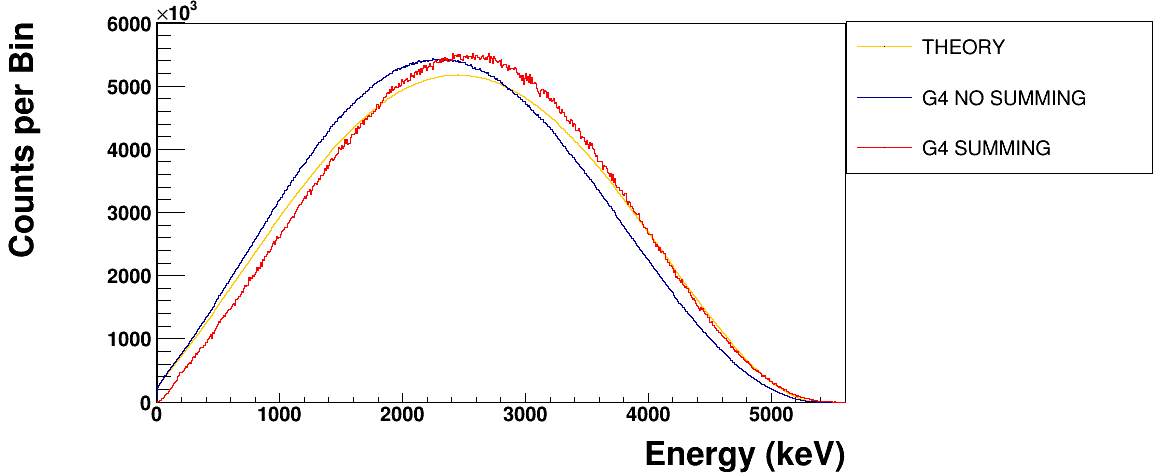
\includegraphics[width=0.78\textwidth]{GEANT4OutputBetter.png}}
	\caption{The shapes of the different histograms from the output of the GEANT4 simulation.
		 The input beta spectrum is also plotted.
		 The histograms are put to the same scale.}
	\label{fig:GEANT4Hists}
\end{figure}

These two histograms were built for each of the four different inputs that were needed for the proper shape fit. 
This structure was informed by testing the fit method.
The details of the fit of the beta energy spectrum shape is in the next chapter. 

\section{Simulation Development}
The GEANT4 simulation is based on the example TestEm5.
The first changes were to add the proper detector geometry, as described above.
The next changes were to add a second primary particle, which was the gamma ray from the decay curve.
The data structure that recorded all the data absorbed event by event was added, so that the gamma cuts could be changed after the fact.

Initially, all energy absorbed by the implant was recorded, regardless of its origin.
This was found not to be the correct way to fit the data.
To counteract that, the class G4VUserTrackInformation was implemented.
This gave the each track the information about the primary particle.
To split the energies from different detectors, the initial energy and charge of each primary particle was checked.
Since the gamma rays are mono-chromatic, the energy of the primary particle was compared to 1.6336 MeV.
If the primary particle had charge or it was a photon without an initial energy of 1.6336 MeV, it was put in the category of energy from the initial electron. 
This took care of most cases, unless a sampled inner bremsstrahlung photon had exactly that energy, which was rare enough to be negligible.

The radiative correction used was changed.
Initially, it was assumed that all the real photons generated by the radiative correction would be absorbed.
It was also assumed that the higher energy inner bremsstrahlung would not come in large enough numbers to have an appreciable effect. 
This would make the radiative correction in equation \ref{eq:fayansrad} adequate. 
However, after explicitly generating the inner bremsstrahlung photons, this was found not to be true.
Therefore, the entire simulation had to be rerun with the inner bremsstrahlung photons generated explicitly.

Then, it was discovered that only running one simulation was not the correct way of fitting the data.
Initially, the corrected phase space without the shape factor was fed into the GEANT4 Monte Carlo.
Then, during the fitting, the shape factor multiplied the output. 
This was found not to be correct, so four simulations were needed.
The simulations were the phase space times the pieces of the shape factor.
This was an issue, as the first version of the code took a week to run 2e9 events.
To speed up the code, the code was modified to use GEANT4 MPI parallelization.
The code was then run on the fireside cluster at the NSCL.
After modification, it only took 6 hours to run 2e9 events.

\subsection{Detector Geometry Changes}
The detector geometry itself was adjusted several times.
Initially, the implant detector was just left as a CsI crystal without any dead layer or cans.
This crystal was 50 mm by 50 mm by 97.6 mm.
This size was given from the group that uses the detectors for $\gamma$ spectroscopy.
The four gamma detectors initially had CsI crystals that were 75.5 mm by 75.5 mm by 72.2 mm in size.
These crystals were surrounded by 2 mm of vacuum, which was supposed to model a dead layer.
After the dead layer, the crystal was surrounded by 1.5 mm of MgO on the sides.
The two sides along the short dimension was left open.
A 1 mm Al can surrounded the crystal, and was also open on the sides.
Both the can and the MgO layer were offset.

After that geometry, the implant's geometry was updated to match the gamma detectors' geometries more closely.
A 2 mm gap was added, and then surrounded by 1.5 mm of MgO. 
On top of that, a 1 mm layer of Al was added.
However, the top and bottom of the detector was left bare in the MgO powder and the Al layer.
This was fixed, and the can and the MgO completely surrounded the detector.

The detector geometry with the MgO is not what the actual detector geometry is.
This geometry was tuned in order to match the efficiency of the data better.
With this tuning, the efficiency is off about 4\% of the measured value. 

It was found that the detector geometry in the simulation has a large effect on the results of the fit.
The final detector geometry was that from technical drawings of the detectors.
This geometry ultimately used  is the one described above. 

\subsection{Data Output Changes}
Another change that was made is in how the simulation results were built.
Initially, all the energy absorbed in each detector was put into a TTree.
This meant that 2e9 events generated 60 GB of output files.
To reduce this space requirement, first only events were any gamma detector had a non-zero input were recorded.
This cut down the space required by 1/3 to 20 GB.
This was not enough, however, as each fit needed four histograms.
A requirement that only one detector fired in order to get the event recorded in the TTree was imposed. 
This cut down the space to 16 GB for 2e9 events.
As the final simulation needed 1.4e10 events, this still was not enough.
However, this last configuration was used to calcuated most of the systematic effects.

Since there is a requirement for only one gamma detector to fire, the gamma-beta coincidences are indepedent detector to detector.
To save space, it is then possible to build 2-D histograms for each of the four gamma detectors.
The energy of the gamma ray was plotted on the x-axis, and the energy absorbed in the implant detector on the y-axis. 
For each detector, two of these histograms were built.
One had the beta-only information.
The other had the information about the beta-gamma sum spectra.
Then, when it came time to apply the beta cuts, the 2-D histogram was projected onto the x-axis and the spectra built.
To check if the binning applied to the histogram distorted the output spectra at all, ratios were of the two output spectra were taken.
The results of the ratios can be seen in figure \ref{fig:histogramtottreeratio}.
The difference is very small.
This method of processing the data was used to test the sensitivity of the fit to the charge radius and the beta end point.

\begin{figure}
    \centering
    \begin{minipage}{0.50\textwidth}
        \centerline{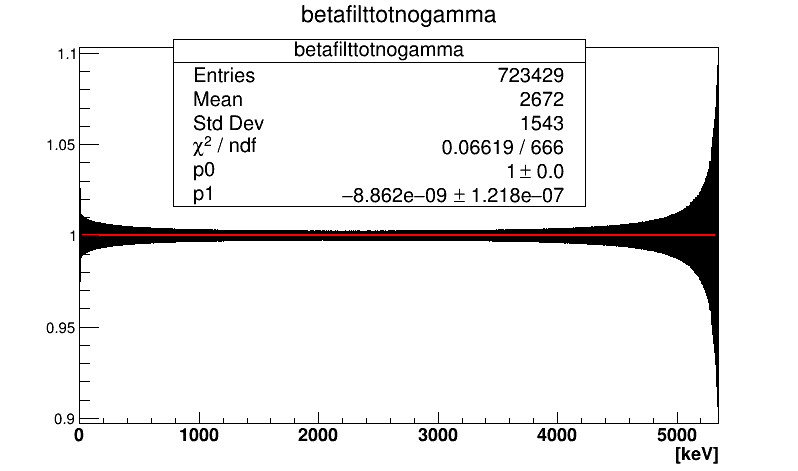
\includegraphics[width=0.9\textwidth]{GEANT42DHistogramsvTTreeFilteredRatio.png}}
    \end{minipage}\hfill
    \begin{minipage}{0.50\textwidth}
        \centerline{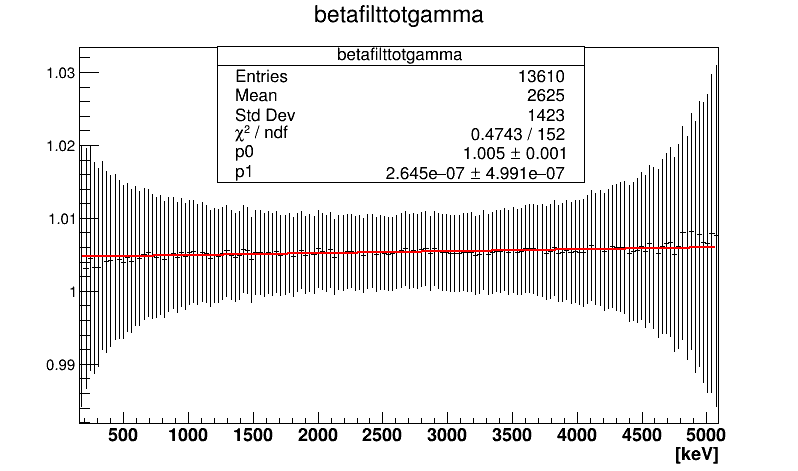
\includegraphics[width=0.9\textwidth]{GEANT42DHistogramsvTTreeFilteredRatio_WithGamma.png}}
    \end{minipage}
    \caption{Ratio of processing data two different ways.
	     Left shows the beta only spectrum ratio.
	     Right shows the sum spectrum.}
    \label{fig:histogramtottreeratio}
\end{figure}

\end{document}
